\chapter{Ausblick}



\section{Kryo-Elektronenmikroskopie}

In dieser Arbeit wurde mit einem relativ kleinen Datensatz an \ac{SNP}s gearbeitet, die Gründe dafür wurden in Kapitel \ref{sec:probleme_mit_dem_datensatz} diskutiert. Als Hauptgrund hat sich herausgestellt, dass zu wenige 3D Strukturen aufgeklärt sind. 

Die Anzahl aller strukturell aufgeklärten Proteine hat sich in den letzten 10 Jahren von 30\% auf 40\% erhöht, im Gegensatz dazu hat sich die Anzahl an bekannten Sequenzen exponentiell vervielfacht. Basierend auf den aktuellen Trends wird erwartet, dass 55\% der strukturellen Abdeckung innerhalb von 15 Jahren erreicht wird \cite{Khafizov.2014}.

Die neusten Entwicklungen in der Chemie, lassen jedoch hoffen, dass in Zukunft zu erwarten ist, dass sehr viel mehr und vor allem hochauflösende 3D Strukturen zu Verfügung stehen. Denn der diesjährige (2017) Nobelpreis in Chemie\footnote{\url{https://www.nobelprize.org/nobel_prizes/chemistry/laureates/2017/announcement.html}
}, mit dem Titel:
\begin{quote}
    ''Für die Entwicklung der Kryo-Elektronenmikroskopie, für die hochauflösende Strukturbestimmung von Biomolekülen in Lösungen.''
\end{quote}
Von Jacques Dubochet, Joachim Frank und Richard Henderson, beschäftigt sich genau mit diesem Thema. So haben sie erfolgreich gezeigt, dass es möglich ist, die 3D Struktur hochauflösend mit einem Kryo-Elektronenmikroskop in der Zelle zu bestimmen.

\begin{quote}
    ''Now there's an explosion in research''
    - Peter Brzezinski
\end{quote}

\begin{figure}
    \centering
    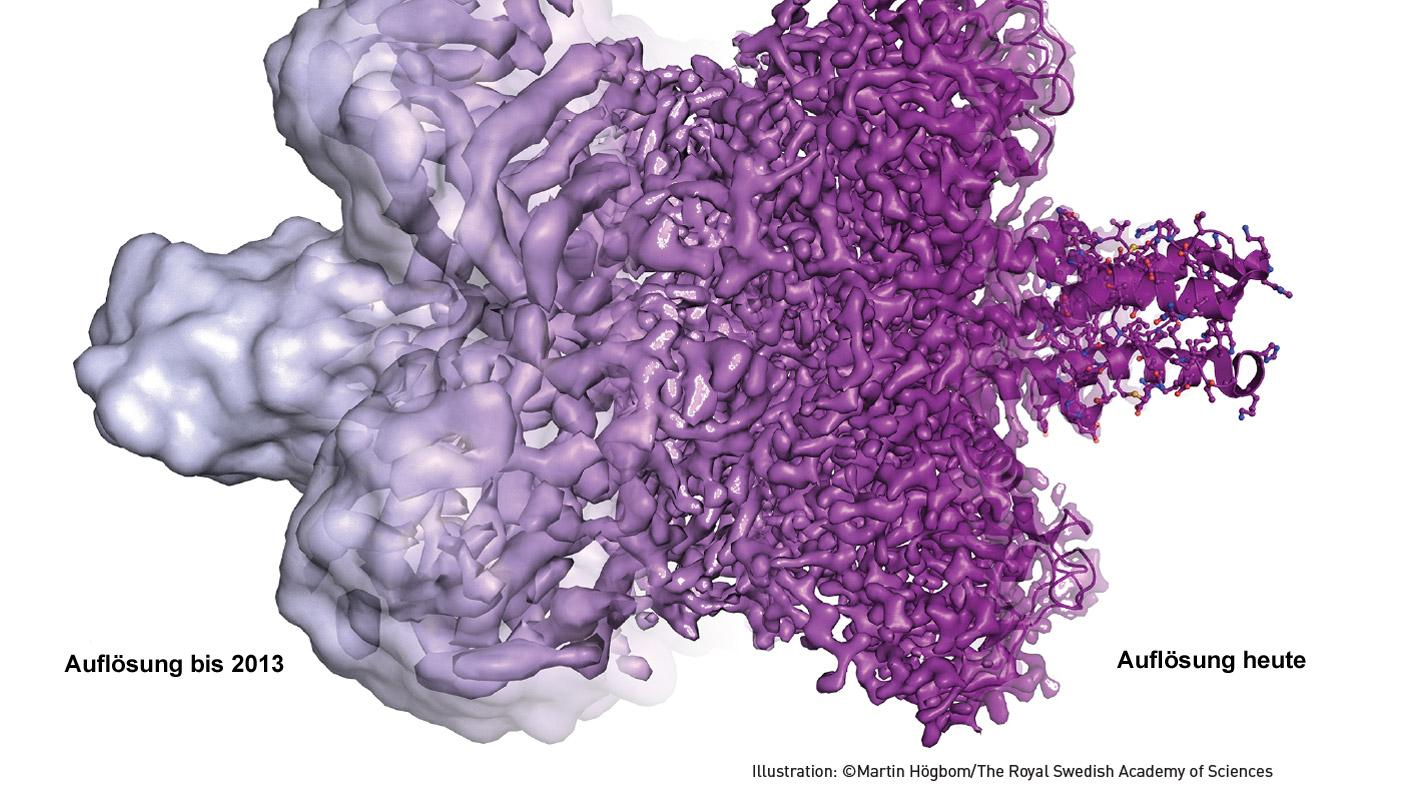
\includegraphics[width=.95\textwidth]{images/Verbesserung_der_Aufloesung.jpg}
    \caption{Verbesserung der Auflösung von 2013 bis heute 2017\protect\footnotemark{}. Die Auflösung war früher gröber, dies ist rechts im Bild dargestellt, heute ist die Auflösung feiner, dies ist rechts in Bild dargestellt. Der Übergang ist beispielhaft in der Mitte gezeigt.}
    \label{fig:verbesserte_aufloesung}
\end{figure}

Bisher war es notwendig das Protein aufzureinigen, um es anschließend in Kristallform zu bringen, da die Röntgenstrukturanalyse nur kristalline Strukturen aufklären kann. 

Die Qualität solcher Strukturen hängt von der Auflösung ab, diese liegt bei 6 bis 2 Angström, das ist links in \ac{Abb} \ref{fig:verbesserte_aufloesung} zu sehen. Die neue Methode ermöglicht es die Strukturen deutlich detailierter darzustellen, wie rechts in der \ac{Abb} gezeigt.

Zusätzlich lassen sich so erstmals Interaktionen zwischen Proteinen direkt unter dem Mikroskop erkennen. Damit kann man auch Proteine in ihren verschiedenen Zuständen beobachten. Das ist auch sehr interessant für diese Arbeit, denn so könnten Energieveränderungen in verschiedenen Konformationen betrachtet werden.
\footnotetext{\url{http://www.blopig.com/blog/wp-content/uploads/2014/04/CootLigand2-624x349.png}}

%" Eine physikalisch korrekte Darstellung molekularer Strukturen erfolgt über die Elektronendichte, welche eine realistische Abbildung des Moleküls in der Realität ist."
%\begin{figure}
%    \centering
%    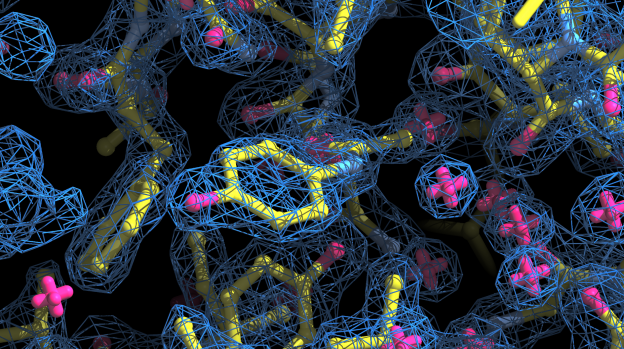
\includegraphics[width=.95\textwidth]{images/approximation.png}
%    \caption{Dargestellt ist eine Approximation der Atome eines Proteins.}
%   \label{fig:approximation}
%end{figure}



\section{Anwendungsgebiete}

Wenden wir uns nun wieder der Thematik der \ac{AML} zu, so sollte es möglich sein alle \ac{SNP}s im Illumina Panel zu annotieren, wenn genug 3D-Strukturen zu Verfügung stehen. Generell ist die Annotation nicht auf das Panel oder den Organismus Mensch beschränkt, sondern lässt sich viel mehr allgemein für jedes Protein verwenden.

Wie in Kapitel \ref{sec:leuk} gezeigt, ist die 5 Jahres Überlebensrate bei \ac{AML} nicht besonders hoch, da die Rückfall Quote nach der Remission sehr hoch ist. 

Um diesen Rückfall rechtzeitig zu erkennen, ist es denkbar nach der Remission spezielle Patienten spezifische pathogene \ac{SNP}s, in regelmäßigen Abständen, im Blut zu suchen. So könnte man früher intervenieren und somit den Rückfall aufhalten, bevor der Patient wieder unter den Symptomen der \ac{AML} leidet.
%\ac{MDS}
Diese \ac{SNP}s im Blut, lassen sich schon in sehr geringer Konzentration nachweisen, noch bevor der Patient wieder die typischen Symptome zeigt. Dies wäre ein weiterer Schritt in Richtung personalisierter Medizin, da das \ac{SNP} Profil für jeden Patienten einzigartig wäre.




\section{Zusammenfassung}
In dieser Arbeit wurde gezeigt, dass sich \acf{APs} zum Annotieren von Single Nucleotide Polymorphisms (SNPs) in Proteinen eignen. Dafür wurden Proteine mit aufgeklärter 3D Struktur untersucht, indem die Aminosäuresequenz mit \ac{SNP}s mutiert wurde. Danach wurden die 3D Strukturen der mutierten Sequenzen zusammen mit der Referenzsequenz, mittels Homologie Modellierung, ermittelt. Für diese Strukturen wurden anschließend Energieprofile (EPs) errechnet, welche danach verglichen wurden.

Dieser Vergleich hat ergeben, dass verschiedene \ac{SNP}s sich unterschiedlich auf das Energieniveau im \ac{EP} auswirken. Des Weiteren wurde gezeigt, dass pathogene \ac{SNP}s das Energieniveau deutlich stärker verändern als benign \ac{SNP}s. Nach verschiedenen Klassifizierungsansätzen wurde gezeigt, dass es am sinnvollsten ist globuläre und alpha helicale Membranproteine getrennt zu betrachten. 

Globuläre Proteine wurden nach der totalen Differenz des Energiewertes am \ac{SNP} klassifiziert. So wurde ein MCC von 0,8 ermittelt, wenn die untere Grenze auf 2 und die obere Grenze auf 7 festgesetzt wird. 

Membran assoziierte Proteine wurden nach der Differenz des Energiewertes am \ac{SNP} klassifiziert, hierbei wurde die untere Grenze auf -2,5 und die obere Grenze auf -0,3 festgelegt. Sind die Werte nun unter oder über dieser Grenze, ist anzunehmen, dass es sich um ein pathogenen \ac{SNP} handelt. Hiermit wurde ein MCC von 1 errechnet, allerdings ist anzumerken, dass der Datensatz relativ klein ist.

Generell lässt sich festhalten das momentan noch sehr wenige 3D Strukturen von Proteinen aufgeklärt sind. Dies ist auch der Grund, warum mit diesem Ansatz, keine \ac{AML} assoziierten \ac{SNP}s aus dem Illumina TruSeq Myeloid Sequenzing Panel, annotiert werden konnten.

Dies könnte sich jedoch in den nächsten Jahren ändern, da z.B. der diesjährige Nobelpreis in Chemie für die Entwicklung der Kryo-Elektro\-nen\-mi\-kros\-ko\-pie für die hochauflösende Strukturbestimmung von Biomolekülen in Lösungen vergeben wurde. Damit ist es möglich schneller und günstiger hochauflösende 3D Strukturen zu erfassen, als es bisher der Fall war.



\section{Weiterführende Arbeit}

\subsection{Validierung im Labor}
In einer weiterführenden Arbeit wäre es sinnvoll, ein einzelnes Protein zu untersuchen, zur Bestätigung der in dieser Arbeit formulierten Theorie. Zum Beispiel wäre es möglich ein integrales Membranprotein wie Bacteriorhodopsin, näher zu Untersuchen. Dieses besitzt eine vollständig aufgeklärte 3D-Struktur\footnote{\url{https://www.rcsb.org/pdb/explore.do?structureId=1FBB}}. Zusätzlich gibt es auch strukturell aufgeklärte Mutanten dieses Proteins \cite{Vonck.2000}. So könnten \ac{EP}s für alle Mutanten und die Referenz Struktur berechnet werden und anschließend eine Klassifizierung vorgenommen werden. Diese Vorhersage könnte anschließend im Labor validiert werden, indem man die Mutanten, des Bacteriorhodopsin, auf Funktionalität überprüft.


\subsection{Online Service}
Das Programm eignet sich als Basismodul für eine klinisch Analyse-Pipeline, die der eigentlichen Variantenanalyse nachgeschaltet ist. Außerdem ist es denkbar, dass die in dieser Arbeit erstellen Skripte auf einem online Service gehostet werden, der über jeden Browser erreichbar ist. Dieser Service könnte dann die in dieser Arbeit beschriebenen Funktionen, jedem Nutzer einfach zu Verfügung stellen. %wie z.B. die Annotation von \ac{SNP}s, indem man eine \ac{SNP}